\documentclass{beamer}
\mode<presentation>
\usetheme{CambridgeUS}
\usepackage[russian]{babel}
\usepackage[utf8]{inputenc}
\usepackage[T2A]{fontenc}
\usepackage{sansmathaccent}

\usepackage{verbatim}
\usepackage{alltt}

\pdfmapfile{+sansmathaccent.map}
\title[Язык C]{Управление процессами, часть 6}
\author{Наумов Д.А., доц. каф. КТ}
\date[15.10.2019] {Операционные системы и системное программное обеспечение, 2019}

\begin{document}

%ТИТУЛЬНЫЙ СЛАЙД
\begin{frame}
  \titlepage
\end{frame}
  
%СОДЕРЖАНИЕ ЛЕКЦИИ
\begin{frame}
  \frametitle{Содержание лекции}
  \tableofcontents  
\end{frame}

\section{Основные понятия}

\begin{frame}{Программы, процессы и потоки}
\begin{block}{Бинарный модуль (программа, приложение)}
компилированный, исполняемый код, находящийся в каком-либо хранилище данных, например на диске.
\end{block}
\begin{block}{Процесс}
запущенная программа.
\end{block}
Процесс включает в себя:
\begin{itemize}
\item бинарный образ, загружаемый в память;
\item подгрузку виртуальной памяти;
\item ресурсы ядра (открытые файлы, выполнение требований по безопасности);
\item запуск одного или нескольких потоков.
\end{itemize}
\textbf{Поток} - это одно из действий внутри процесса. Поток
имеет собственный виртуализированный процессор, включающий в себя стек,
состояние процессора, например регистры, а также командные указатели.
\end{frame}

\section{Идентификаторы процессов}

\begin{frame}{Идентификатор процесса}
\begin{block}{Идентификатор процесса (process ID, pid)}
уникальное (в любой конкретный момент времени) число, обозначающее процесс
\end{block}
\begin{itemize}
\item процесс бездействия (idle process) - pid = 0;
\end{itemize}
\begin{block}{Процесс инициализации}
первый процесс, который ядро выполняет во время запуска системы, pid = 1
\end{block}
\begin{itemize}
\item /sbin/init - наиболее вероятное размещение процесса инициализации 
\item /etc/init - следующее вероятное размещение процесса инициализации
\item /bin/init - резервное размещение процесса инициализации
\item /bin/sh - местонахождение оболочки Bourne, которую ядро пытается запустить
\end{itemize}
\end{frame}

\begin{frame}{Идентификатор процесса}
\begin{block}{pid\_t}
С точки зрения программирования идентификатор процесса обозначается типом
pid\_t, величина которого определяется в заголовочном файле <<sys/types.h>>. 
\end{block}
Выделение идентификатора процесса
\begin{itemize}
\item максимальное значение - /proc/sys/kernel/pid\_max
\item идентификаторы назначаются линейно
\item ранее исползованные индентификаторы не назначаются, пока не будет достигнуто pid\_max 
\end{itemize}
\end{frame}

\begin{frame}{Иерархия процессов, пользователи, группы}
Процесс, запускающий другой процесс, называется \textbf{родительским}; новый процесс, таким образом, является \textbf{дочерним}.
\begin{itemize}
\item каждый процесс запускается каким­либо другим процессом (кроме, разумеется, процессов инициализации). 
\item каждый дочерний процесс имеет <<родителя>>. 
\item идентификатор родительского процесса - \textbf{ppid}.
\item каждый процесс принадлежит определенному \textbf{пользователю} и \textbf{группе}. Эти принадлежности используются для управления правами доступа к ресурсам. 
\item каждый дочерний процесс наследует пользователя и группу, которым принадлежал родительский процесс.
\item каждый процесс является также частью \textbf{группы процессов}. Дочерние процессы, как правило, принадлежат к тем же группам процессов, что и родительские.
(Пример: \textit{ls | less}) 
\end{itemize}
\end{frame}

\begin{frame}{Получение идентификатора процесса}
Системный вызов getpid() возвращает идентификатор вызывающего процесса:
\begin{figure}[h]
\centering
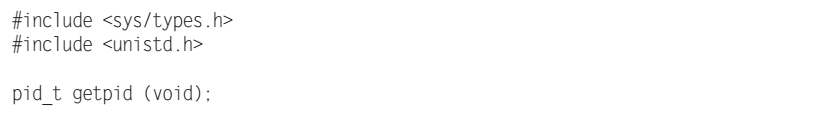
\includegraphics[scale=0.5]{images/lec07-pic01.png}
\end{figure}
Системный вызов getppid() возвращает идентификатор родителя вызывающего процесса:
\begin{figure}[h]
\centering
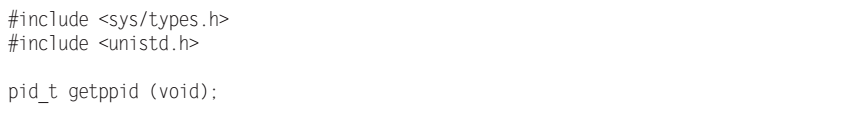
\includegraphics[scale=0.5]{images/lec07-pic02.png}
\end{figure}
Ни один из них не может вернуть ошибку:
\begin{figure}[h]
\centering

\includegraphics[scale=0.5]{images/lec07-pic03.png}
\end{figure}
\end{frame}

\section{Запуск нового процесса}

\begin{frame}{Запуск нового процесса}
В UNIX действие загрузки в память и запуска образа программы выполняется
отдельно от операции по созданию нового процесса:
\begin{itemize}
\item один системный вызов (exec) загружает бинарную программу в память, замещая текущее содержание адресного пространства, и начинает выполнение новой программы. 
\item другой системный вызов (fork) используется для создания нового процесса, который изначально является практически копией своего родительского.
\end{itemize}
\end{frame}

\begin{frame}{Семейство вызовов exec}
Единой функции exec не существует; на одном системном вызове построено целое
семейство таких функций. Рассмотрим execl:
\begin{figure}[h]
\centering
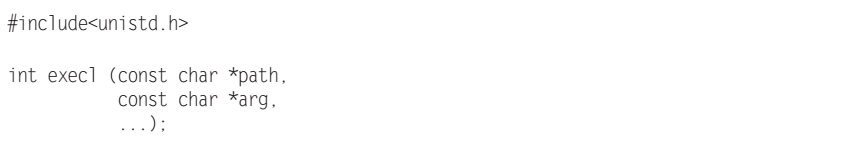
\includegraphics[scale=0.5]{images/lec07-pic04.png}
\end{figure}
\begin{itemize}
\item вызов execl() замещает текущий образ процесса новым, загружая в память
программу, определенную path. 
\item параметр arg — первый аргумент этой программы. 
\item Многоточие означает переменное количество аргументов — у функции
execl() их количество может быть любым
\item дополнительные аргументы можно указывать в скобках один за другим
\item список аргументов всегда завершается значением NULL.
\end{itemize}
\end{frame}

\begin{frame}{Семейство вызовов exec}
Следующий программный код замещает выполняющуюся в настоящий момент программу с /bin/vi:
\begin{figure}[h]
\centering
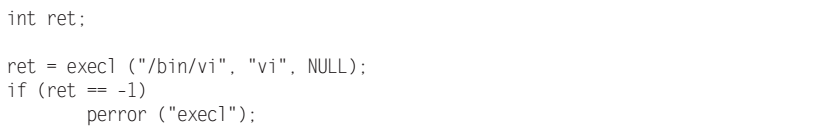
\includegraphics[scale=0.5]{images/lec07-pic05.png}
\end{figure}
Если вы хотите редактировать файл /home/kidd/hooks.txt, то должны запустить следующий код:
\begin{figure}[h]
\centering
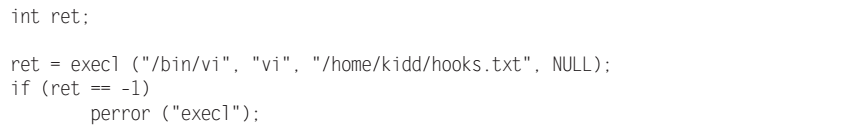
\includegraphics[scale=0.5]{images/lec07-pic06.png}
\end{figure}
\end{frame}

\begin{frame}{Семейство вызовов exec}
\begin{itemize}
\item при успешном вызове execl() не возвращает никаких значений 
\item если произошла ошибка, execl() возвращает –1 и устанавливает errno.
\end{itemize}
В случае успешного выполнения вызов execl():
\begin{itemize}
\item изменяет адресное пространство и образ процесса;
\item любые ожидающие сигналы исчезают;
\item любые сигналы, отлавливаемые процессом, возвращаются к своему
поведению по умолчанию;
\item все блокировки памяти удаляются;
\item большинство атрибутов потока возвращается к значениям по умолчанию;
\item большая часть статистических данных процесса сбрасывается;
\item все адресное пространство памяти, относящееся к данному процессу, включая
загруженные файлы, очищается.
\end{itemize}
\end{frame}

\begin{frame}{Семейство вызовов exec}
\begin{itemize}
\item execl, execlp, execle  
\item execv, execvp, execve
\end{itemize}
<<Расшифровка>> названий функций:
\begin{itemize}
\item \textbf{l} и \textbf{v} указывают, передаются ли аргументы списком или массивом. 
\item \textbf{p} указывает, что система будет искать указанный файл по
полному пользовательскому пути. 
\item \textbf{е} обозначает, что для нового процесса создается новое окружение.
\end{itemize}
\end{frame}

\begin{frame}{Системный вызов fork()}
Новый процесс, запускающий тот же системный образ, что и текущий, может быть
создан с помощью системного вызова fork():
\begin{figure}[h]
\centering

\includegraphics[scale=0.5]{images/lec07-pic07.png}
\end{figure}
\begin{itemize}
\item В случае успешного обращения к fork() создается новый процесс, во всех отношениях идентичный вызывающему. 
\item Оба процесса выполняются от точки обращения к fork(), как будто ничего не происходило.
\end{itemize}
\end{frame}

\begin{frame}{Системный вызов fork()}
В дочернем процессе успешный запуск \textbf{fork()} возвращает \textbf{0}. В родительском \textbf{fork()} возвращает \textbf{pid} дочернего. 

Родительский и дочерний процессы практически идентичны, за исключением некоторых особенностей:
\begin{itemize}
\item pid дочернего процесса назначается заново и отличается от родительского;
\item родительский pid дочернего процесса установлен равным pid родительского
процесса;
\item ресурсная статистика дочернего процесса обнуляется;
\item любые ожидающие сигналы прерываются и не наследуются дочерним процессом;
\item никакие вовлеченные блокировки файлов не наследуются дочерним процессом.
\end{itemize}
\end{frame}

\begin{frame}{Системный вызов fork()}
В случае ошибки дочерний процесс не создается, fork() возвращает –1, устанавливая соответствующее значение errno. 

Вот два возможных значения errno и их
смысл:
\begin{itemize}
\item EAGAIN — ядро не способно выделить определенные ресурсы, например новый
pid, или достигнуто ограничение по ресурсам RLIMIT\_NPROC;
\item ENOMEM — недостаточно ресурсов памяти ядра, чтобы завершить запрос.
\end{itemize}
\begin{figure}[h]
\centering
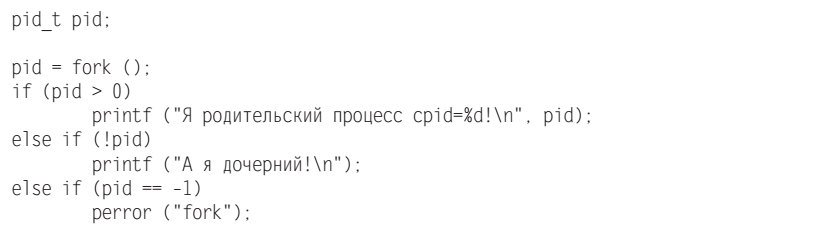
\includegraphics[scale=0.5]{images/lec07-pic08.png}
\end{figure}
\end{frame}

\begin{frame}{Системный вызов fork()}
Чаще всего системный вызов fork() используется для создания нового процесса
и последующей загрузки в него нового двоичного образа.  Сначала процесс ответвляет новый процесс, а потом дочерний процесс создает новый двоичный образ.
\begin{figure}[h]
\centering
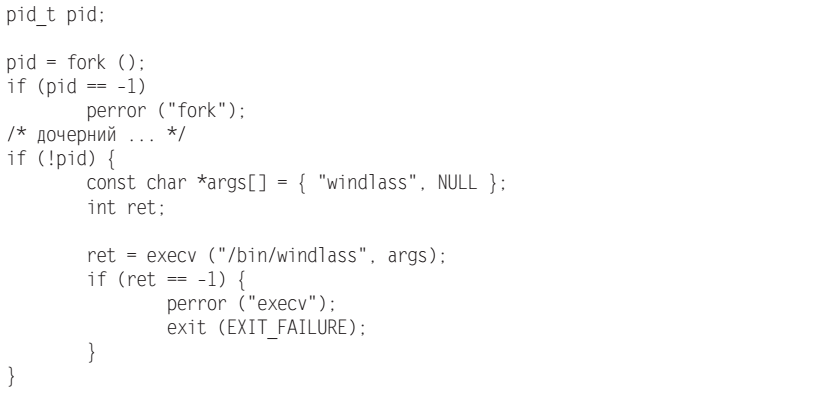
\includegraphics[scale=0.5]{images/lec07-pic09.png}
\end{figure}
\end{frame}

\section{Завершение процесса}

\begin{frame}{Завершение процесса}
POSIX и C89 определяют следующую стандартную функцию для завершения текущего процесса:
\begin{itemize}
\item вызов exit() выполняет некоторые основные шаги перед завершением, а затем
отправляет ядру команду прекратить процесс.
\item параметр status используется для обозначения статуса процесса завершения.
\item значения EXIT\_SUCCESS и EXIT\_FAILURE определяются в качестве способов представления успеха и неудачи. 
\end{itemize}
Перед тем как прервать процесс, библиотека C выполняет подготовительные
шаги в следующем порядке.
\begin{enumerate}
\item Вызов всех функций, зарегистрированных с atexit() или on\_exit(), в порядке,
обратном порядку регистрации.
\item Сброс всех стандартных потоков ввода­вывода.
\item Удаление всех временных файлов, созданных функцией tmpfile().
\end{enumerate}
\end{frame}

\begin{frame}{Завершение процесса}
Другие способы завершения:
\begin{itemize}
\item <<достижение конечной точки>> программы (системный выхов exit - неявный);
\item полезно возвращать статус выхода явно;
\item процесс также может завершиться, если ему отправлен сигнал, действие которого по умолчанию — окончание процесса (SIGTERM и SIGKILL);
\item ядро может прервать процесс, выполняющий недопустимые инструкции, нарушающий сегментацию, исчерпавший ресурсы памяти и т. д.
\end{itemize}
\end{frame}




\end{document}
 